% ============================================================================
% TÀI LIỆU THAM KHẢO
% ============================================================================
\section*{TÀI LIỆU THAM KHẢO}
\addcontentsline{toc}{section}{TÀI LIỆU THAM KHẢO}

\begingroup
\raggedright
\begin{enumerate}[label={[\arabic*]}, leftmargin=2.2em, itemsep=3pt]
    \item P. Lewis \textit{et al.}, ``Retrieval-augmented generation for knowledge-intensive NLP tasks,'' in \textit{Proc. Advances in Neural Information Processing Systems (NeurIPS)}, vol. 33, pp. 9459--9474, 2020.
    \item S. Robertson and H. Zaragoza, ``The probabilistic relevance framework: BM25 and beyond,'' \textit{Foundations and Trends in Information Retrieval}, vol. 3, no. 4, pp. 333--389, 2009.
    \item V. Karpukhin \textit{et al.}, ``Dense passage retrieval for open-domain question answering,'' in \textit{Proc. Conf. Empirical Methods in Natural Language Processing (EMNLP)}, pp. 6769--6781, 2020.
    \item Y. Zhang \textit{et al.}, ``Qwen3 Embedding: Advancing text embedding and reranking through foundation models,'' \textit{arXiv preprint arXiv:2506.05176}, 2025.
    \item A. Kusupati \textit{et al.}, ``Matryoshka representation learning,'' in \textit{Proc. Advances in Neural Information Processing Systems (NeurIPS)}, vol. 35, pp. 30233--30249, 2022.
    \item G. V. Cormack, C. L. A. Clarke, and S. Buettcher, ``Reciprocal rank fusion outperforms condorcet and individual rank learning methods,'' in \textit{Proc. 32nd Int. ACM SIGIR Conf. Research and Development in Information Retrieval}, pp. 758--759, 2009.
    \item R. Nogueira and K. Cho, ``Passage re-ranking with BERT,'' \textit{arXiv preprint arXiv:1901.04085}, 2019.
    \item W. Wang \textit{et al.}, ``MiniLMv2: Multi-head self-attention relation distillation for compressing pretrained transformers,'' in \textit{Findings of the Association for Computational Linguistics: ACL-IJCNLP}, pp. 2140--2151, 2021.
    \item S. Zhou \textit{et al.}, ``DocPrompting: Generating code by retrieving the docs,'' in \textit{Proc. Int. Conf. Learning Representations (ICLR)}, 2023.
    \item Z. T. Wang \textit{et al.}, ``CodeRAG-Bench: Can retrieval augment code generation?,'' in \textit{Findings of the Association for Computational Linguistics: NAACL}, 2025.
    \item Y. Zhang \textit{et al.}, ``cAST: Enhancing code retrieval-augmented generation with structural chunking via abstract syntax tree,'' \textit{arXiv preprint arXiv:2506.15655}, 2025.
    \item Anthropic, ``Introducing Contextual Retrieval,'' Anthropic Engineering Technical Report, Sep. 2024.
    \item D. Edge \textit{et al.}, ``From local to global: A graph RAG approach to query-focused summarization,'' \textit{arXiv preprint arXiv:2404.16130}, 2024.
    \item Anthropic, ``Model Context Protocol (MCP) Specification,'' \url{https://modelcontextprotocol.io}, 2024.
\end{enumerate}
\endgroup

% ============================================================================
% PHỤ LỤC
% ============================================================================
\section*{PHỤ LỤC}
\addcontentsline{toc}{section}{PHỤ LỤC}

\begin{itemize}
    \item \textbf{Kho mã nguồn mở của dự án:} \url{https://github.com/Hoang604/rag-nlp} cung cấp toàn bộ mã nguồn, PostgreSQL/pgvector database schema, benchmark corpus và hướng dẫn reproduce môi trường qua Docker Compose và trình quản lý gói \texttt{uv}.
    \item \textbf{Đặc tả API của 6 MCP tools chuẩn [14] (hỗ trợ cả \texttt{stdio} và Warm Streamable HTTP \texttt{POST /api/mcp}):}
    \begingroup
    \raggedright
    \begin{enumerate}
        \item \texttt{hybrid\_search(query, \allowbreak pattern, \allowbreak limit, \allowbreak path\_prefix, \allowbreak doc\_slugs, \allowbreak is\_regex, \allowbreak case\_sensitive, \allowbreak rerank)}: Thực thi dual-channel retrieval kết hợp Hybrid RRF + Cross-Encoder Reranking với verbatim/regex matching, trả về các context groups đã sắp xếp theo reading order và confidence label $\gamma$.
        \item \texttt{hierarchical\_navigate(path, \allowbreak direction, \allowbreak limit)}: Duyệt cây phân cấp \texttt{ltree} theo 4 hướng \texttt{CHILDREN}, \texttt{PARENT\_CHAIN}, \texttt{SIBLINGS}, \texttt{SUBTREE} kèm cơ chế tự động tái tạo các virtual parent nodes khi mục cha chỉ đóng vai trò container.
        \item \texttt{graph\_traverse(source\_path, \allowbreak direction, \allowbreak max\_depth, \allowbreak filter\_relations, \allowbreak limit\_per\_link)}: Duyệt đệ quy Knowledge Graph theo hướng \texttt{OUTGOING}, \texttt{INCOMING}, \texttt{BOTH}, tự động xử lý các quan hệ đối xứng và phân bổ quota kết quả công bằng cho từng liên kết.
        \item \texttt{graph\_curate\_edges(reason, \allowbreak add\_edges, \allowbreak remove\_edges)}: Thêm hoặc xóa trong một atomic transaction các graph edges kèm kiểm chứng whitespace-invariant citation grounding, mở rộng container target node xuống các leaf nodes và ghi append-only audit log.
        \item \texttt{get\_raw(path\_or\_slug, \allowbreak start\_line, \allowbreak end\_line)}: Trích xuất nguyên văn line slice $[s, e]$ với giới hạn tối đa 200 dòng mỗi lần gọi trực tiếp từ raw text của tài liệu.
        \item \texttt{submit\_grounded\_answer(answer, \allowbreak citations, \allowbreak abstained)}: Xác thực câu trả lời của \texttt{Agent} bằng cách kiểm tra từng trích dẫn \texttt{(path, start\_line, end\_line)} trực tiếp trên PostgreSQL, trích xuất văn bản nguyên gốc và từ chối ngay lập tức nếu đường dẫn \texttt{ltree} không tồn tại trong kho ngữ liệu.
    \end{enumerate}
    \endgroup
    \item \textbf{Giao diện Corpus \& Graph Observatory Dashboard (\texttt{uv run rag-eval ui}):} Cung cấp cây thư mục tài liệu và \texttt{ltree} trực quan, chế độ xem đối chiếu raw text theo dòng, bản đồ Knowledge Graph 2D hiển thị in-degree/out-degree của từng node, giao diện thử nghiệm Venn retrieval và không gian \textbf{Hỏi đáp có kiểm chứng trích dẫn (Grounded Agent Q\&A)} hiển thị trực tiếp tiến trình gọi công cụ MCP theo thời gian thực qua WebSocket (\texttt{/api/qa/ws}) cùng thẻ đối chiếu văn bản nguyên gốc cho từng dấu trích dẫn \texttt{[\#k]} (Hình \ref{fig:ui_dashboard}).
    \item \textbf{Mẫu các ca kiểm thử tiêu biểu từ bộ dữ liệu \nolinkurl{data/eval/retrieval.jsonl}:} Bảng \ref{tab:sample_queries} trích dẫn 6 ca kiểm thử đại diện cho hai bộ \texttt{TS1-Lexical-API} và \texttt{TS2-Conceptual} trên hai miền Next.js và Node.js, minh họa rõ vai trò của từng phân vùng Venn (\texttt{both}, \texttt{semantic\_only}, \texttt{verbatim\_only}).
\end{itemize}

\begin{figure}[H]
\centering
\begin{minipage}[t]{0.485\textwidth}
    \centering
    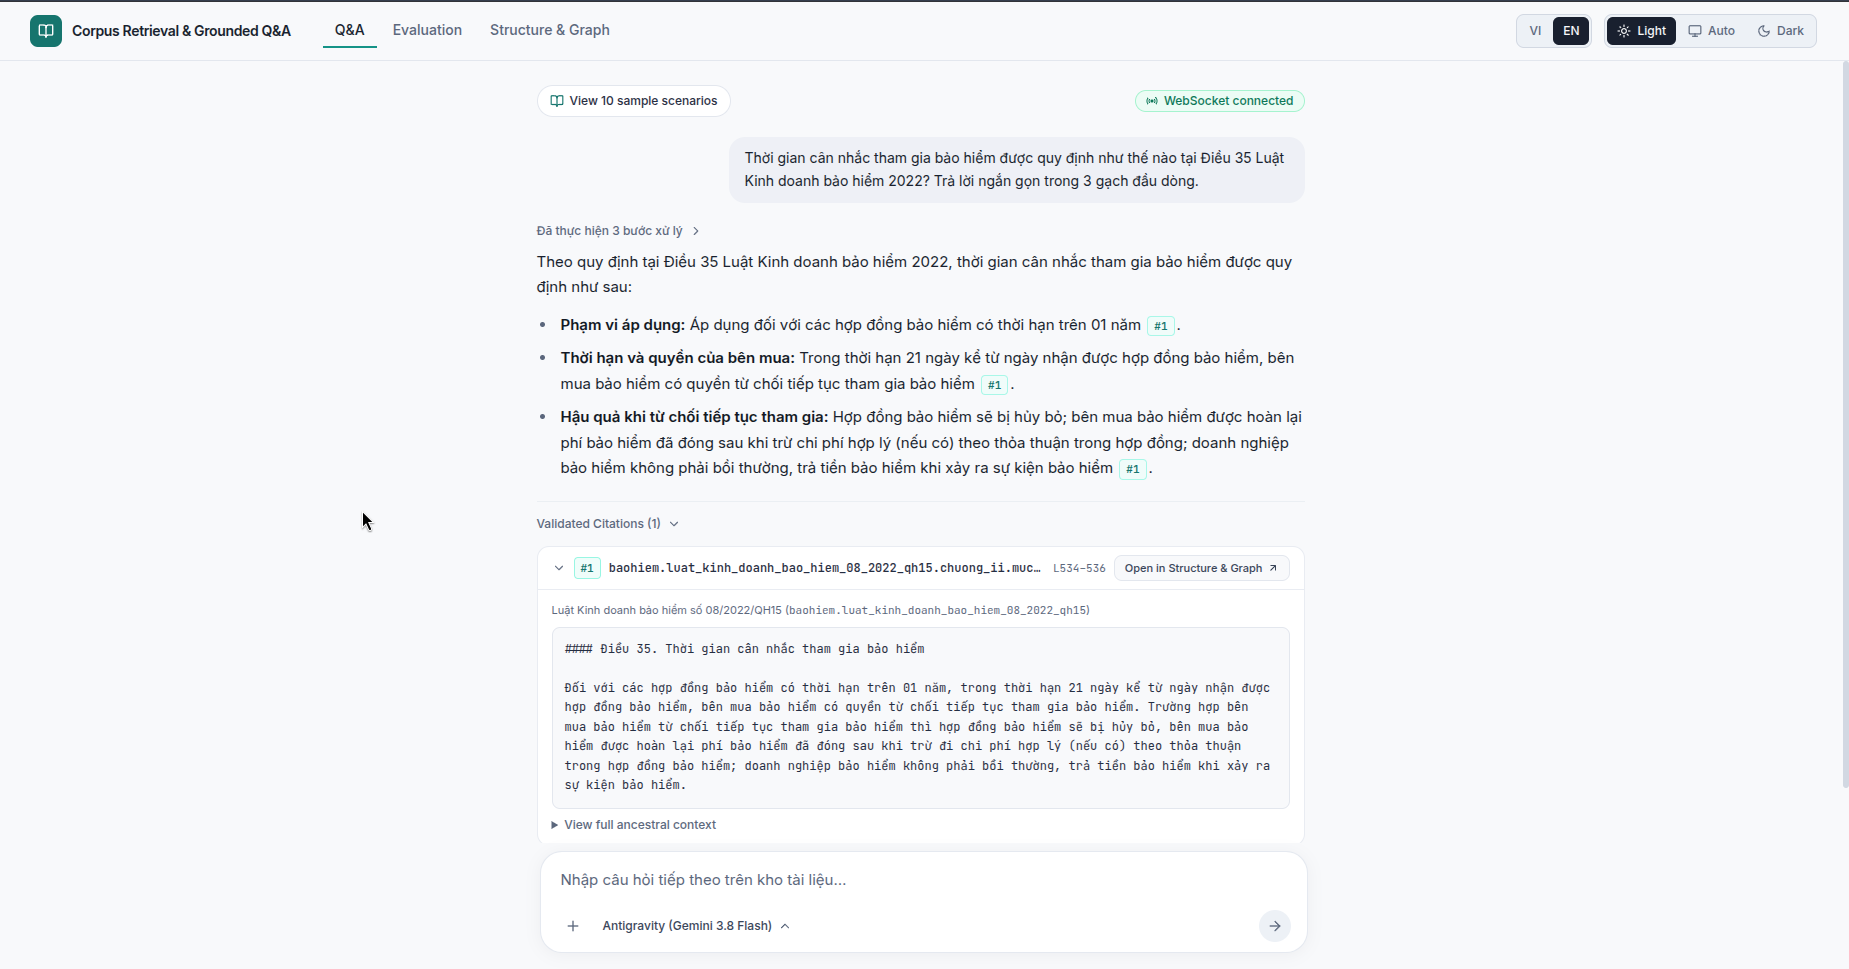
\includegraphics[width=\textwidth]{figures/ui_grounded_qa.png}
    \par\vspace{2pt}{\footnotesize (a) Không gian Hỏi đáp có kiểm chứng trích dẫn (\texttt{Grounded Q\&A}) và luồng sự kiện MCP}
\end{minipage}\hfill
\begin{minipage}[t]{0.485\textwidth}
    \centering
    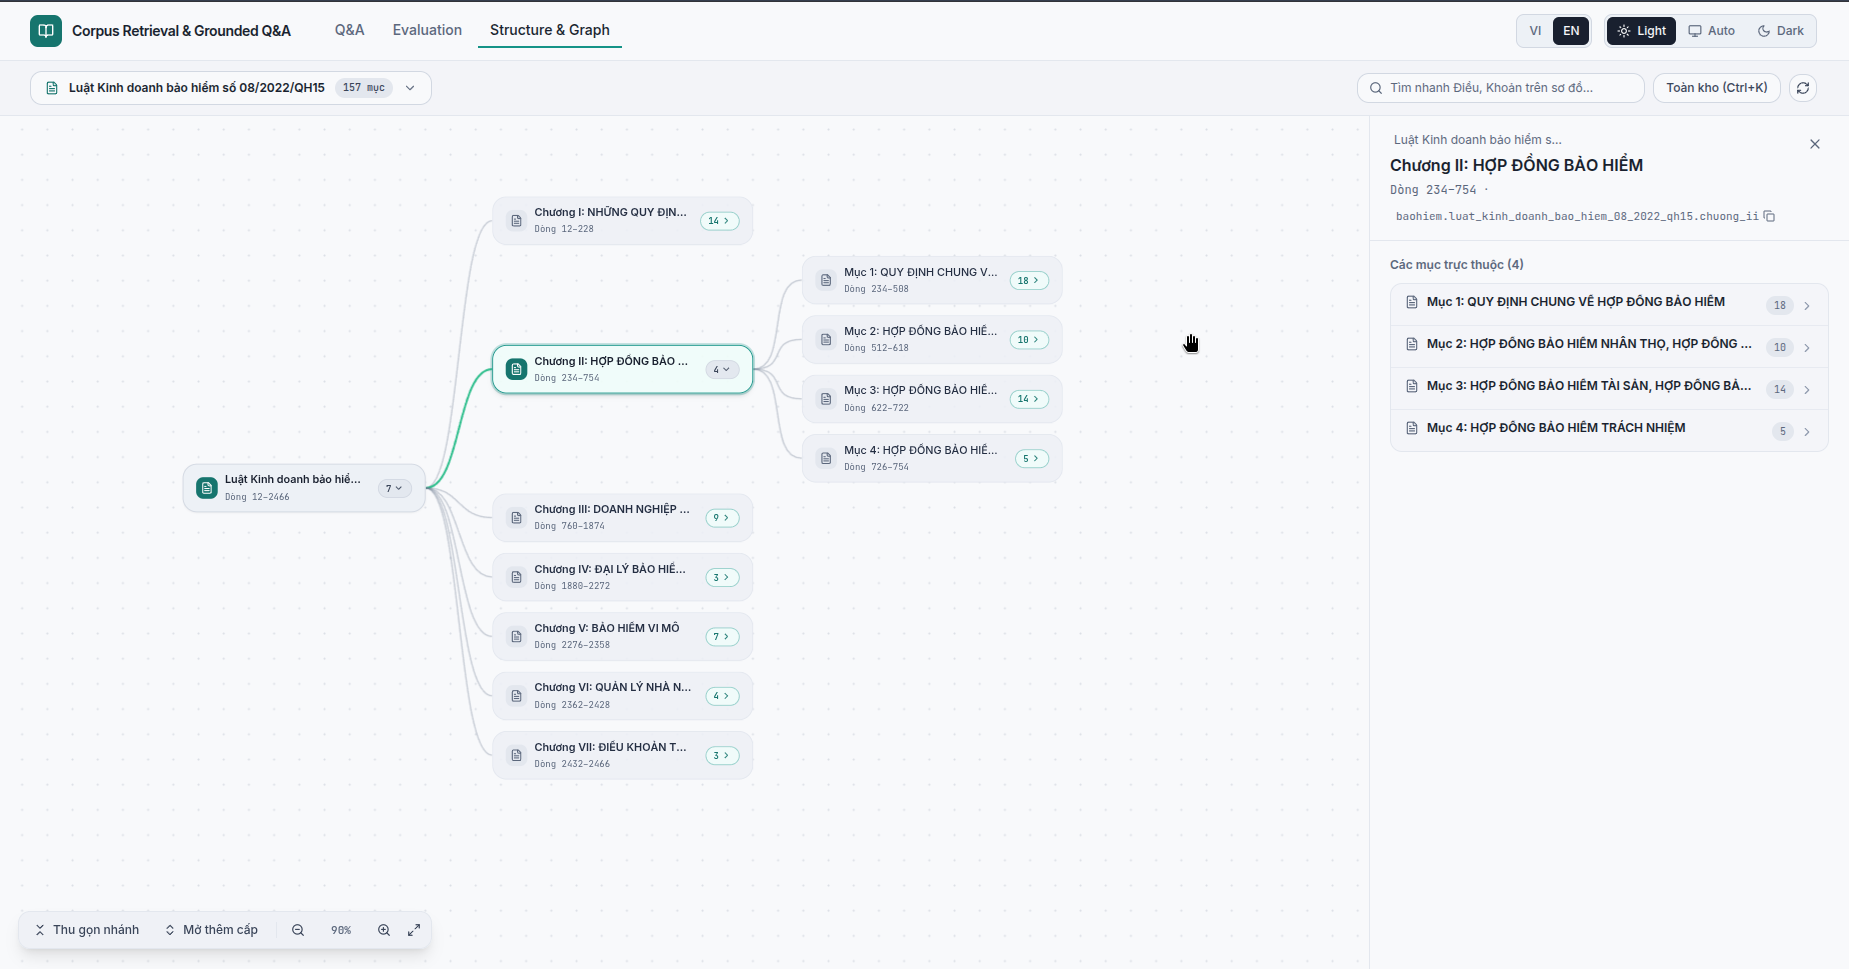
\includegraphics[width=\textwidth]{figures/ui_explorer_graph.png}
    \par\vspace{2pt}{\footnotesize (b) Không gian khám phá cây phân cấp \texttt{ltree}, đối chiếu dòng nguyên bản 1:1 và Knowledge Graph}
\end{minipage}
\caption{Giao diện thực tế của hệ thống Corpus \& Graph Observatory Dashboard (\texttt{uv run rag-eval ui})}
\label{fig:ui_dashboard}
\end{figure}

\begin{table}[H]
\centering
\caption{Mẫu 6 truy vấn kiểm thử tiêu biểu trong bộ đánh giá 100 câu}
\label{tab:sample_queries}
\scriptsize\setlength{\tabcolsep}{3.5pt}\begin{tabularx}{\textwidth}{ll>{\raggedright\arraybackslash}X>{\raggedright\arraybackslash}p{3.0cm}>{\raggedright\arraybackslash}p{3.9cm}c}
\toprule
\textbf{Mã} & \textbf{Bộ / Miền} & \textbf{Câu hỏi tóm tắt} & \textbf{\texttt{query} / \texttt{pattern}} & \textbf{Đường dẫn \texttt{ltree} đích} & \textbf{Giỏ / Hạng} \\
\midrule
\texttt{e001} & \texttt{TS1}\newline Next.js & Cờ \texttt{--yes} của \texttt{create-next-app} cấu hình mặc định import alias và bundler nào? & \texttt{create-next-app --yes...}\newline\texttt{pattern: "--yes"} & \nolinkurl{nextjs.01_getting_started.01_installation.quick_start} & \texttt{both}\newline (\#1) \\
\addlinespace[2pt]
\texttt{e021} & \texttt{TS1}\newline Next.js & Truyền \texttt{FormData} của Server Action vào \texttt{Object.fromEntries} sinh ra các thuộc tính nội bộ có tiền tố gì? & \texttt{Server Action FormData...}\newline\texttt{pattern: "\$ACTION"} & \nolinkurl{nextjs.02_guides.forms.how_it_works} & \texttt{verbatim}\newline (\#1) \\
\addlinespace[2pt]
\texttt{e029} & \texttt{TS1}\newline Node.js & Trên Windows, khi \texttt{options.env} của \texttt{spawn} chứa cả khóa \texttt{PATH} và \texttt{Path}, Node.js chọn khóa nào? & \texttt{child\_process spawn...}\newline\texttt{pattern: "options.env"} & \nolinkurl{nodejs.child_process.overview} & \texttt{both}\newline (\#1) \\
\addlinespace[2pt]
\texttt{e053} & \texttt{TS2}\newline Next.js & Vì sao triển khai nhiều replica Next.js tự host gây lỗi \texttt{Failed to find Server Action} và cần biến môi trường nào? & \texttt{self-hosting multiple...}\newline\texttt{pattern: "NEXT\_SERVER\_..."} & \nolinkurl{nextjs.02_guides.self_hosting.multi_server_deployments.server_functions_encryption_key} & \texttt{both}\newline (\#1) \\
\addlinespace[2pt]
\texttt{e072} & \texttt{TS2}\newline Next.js & Trong kiến trúc Multi-Zones, vì sao liên kết giữa các zone phải dùng thẻ \texttt{<a>} và tránh đụng độ tài nguyên tĩnh thế nào? & \texttt{Multi-Zones links...}\newline\texttt{pattern: "assetPrefix"} & \nolinkurl{nextjs.02_guides.multi_zones.linking_between_zones} & \texttt{semantic}\newline (\#2) \\
\addlinespace[2pt]
\texttt{e083} & \texttt{TS2}\newline Node.js & Sau khi monkey-patch CommonJS export của \texttt{node:fs}, làm sao đồng bộ lại các named exports bên ES module? & \texttt{syncBuiltinESM...}\newline\texttt{pattern: "syncBuiltin..."} & \nolinkurl{nodejs.module.the_module_object.module_syncbuiltinesmexports} & \texttt{verbatim}\newline (\#1) \\
\bottomrule
\end{tabularx}
\end{table}

\vspace{0.3cm}
\begin{center}
\begin{tabular}{p{0.45\textwidth}p{0.45\textwidth}}
\centering \textbf{GIẢNG VIÊN HƯỚNG DẪN} & \centering\arraybackslash \textbf{ĐẠI DIỆN NHÓM THỰC HIỆN} \\
\centering \textit{Ký và ghi rõ họ tên} & \centering\arraybackslash \textit{Ký và ghi rõ họ tên} \\[1.8cm]
\centering \textbf{ThS. Nguyễn Văn Sơn} & \centering\arraybackslash \textbf{Đinh Việt Hoàng}
\end{tabular}
\end{center}
